%%%%%%%%%%%%%%%%%%%%%%%%%%%%%%%%%%%%%%%%%%%%%%%%%%%%%%%%%%%%%%%%%%%%%%%%
\chapter{Methods} \label{chap:Methods}
%%%%%%%%%%%%%%%%%%%%%%%%%%%%%%%%%%%%%%%%%%%%%%%%%%%%%%%%%%%%%%%%%%%%%%%%
\vspace{1cm}

This chapter describes the methods employed in the present work for fetal brain MRI segmentation and evaluation. The focus is on the domain generalization of deep learning models.

It starts with an overview of nnU-Net, a self-configuring U-Net-based framework that has become a widely adopted baseline in medical image segmentation. Building on this baseline, the method \textsc{gin-ipa} is introduced as an augmentation strategy to enhance domain generalization. Finally, to objectively assess model performance a set of evaluation metrics is presented, based on segmentation accuracy. These include overlap-based measures such as the Dice coefficient, as well as surface-distance-based metrics that capture geometric fidelity.

\section{nnU-Net} \label{sec:nnUNet}
nnU-Net\,\cite{Isensee2021, nnUNet} is an automated pipeline for the tissue segmentation in a task-agnostic configuration, that is, nnU-Net is designed to be applicable to a wide variety of target structures and image properties. Its self-configuring nature allows it to be applied to arbitrary new datasets without manual intervention. Actually, nnU-Net does not introduce new elements in the network architecture, but by systematizing the complex process of manual tuning it manages to achieve an automated and efficient setting of parameters in U-Net architecture. This generalized choice of pipeline parameters is carried out based on a \enquote{dataset fingerprint}, that is \enquote{a standardized dataset representation comprising key properties}\,\cite{Isensee2021} of the images. The parameter setting strategy is based on distinguishing between three classes of parameters that can be optimized:
\begin{description}
    \item[Fixed parameters] A robust and consistent choice of hyperparameters and design implementation that is suitable for any task and dataset---they can still be manually changed though. Examples are learning rate, loss function, optimizer, training and testing procedure.
    \item[Rule-based parameters] They are set based on the information taken from the dataset fingerprint, which is acquired during the preprocessing step. This information is fed into rules to automatically make several choices, such as patch and batch size, network topology, intensity normalization, and resampling strategy.
    \item[Empirical parameters] Limited to the choice of the U-Net configuration (2D, 3D-fullres, 3D-cascade) and post-processing.
\end{description}
The rules established generate the same set of parameters and architecture when the image size and the pixel spacing are the same or similar. Default preprocessing consists in cropping the image around non-zero voxels and performing \textit{z}-normalization.

Data augmentation in nnU-Net consists of a set of standard transformations, that are: flip, rotation, scaling, Gaussian noise and blur, resolution reduction, brightness and contrast adjustments, and gamma transformation\,\cite{nnUNet}. Each transformation is applied randomly with a predetermined, empirically chosen probability\,\cite{Isensee2021}.

nnU-Net is currently one of the most popular tools for MRI fetal brain tissue segmentation, representing the state of the art in this field. Nevertheless, like other methods it suffers drops in performance, especially when it comes to inference on out-of-domain (OOD) images and on specific labels, like ventricles, gray matter and white matter.

\section{GIN-IPA} \label{sec:gin-ipa}
To improve robustness of segmentation models against acquisition-induced domain shifts, the causality-inspired augmentation pipeline \textsc{gin-ipa}\,\cite{Ouyang2023} was adopted. The method, that is aimed at single-source domain generalization (see Section \ref{sec:DomainGeneralization}), treats the image formation process as generated by two independent factors, acquisition $A$ and content $C$, and seeks to enforce that the segmentation predictor be invariant to interventions on $A$. Concretely, following the causal formulation, the desired invariance can be expressed as
\begin{equation}\label{eq:domain-inv}
    p\bigl(Y\mid S,\,\mathrm{do}(A= a_i)\bigr) 
    = p\bigl(Y\mid S,\,\mathrm{do}(A= a_j)\bigr), \quad \forall a_i,a_j,
\end{equation}
where $S$ denotes an ideal, domain-invariant representation determined by content $C$---i.e., shape information---and $Y$ is the segmentation mask. $p\bigl(Y\mid S,\,\mathrm{do}(A= a_i)\bigr)$ denotes the distribution that comes from letting images to be generated from a specific acquisition process $A = a_i$---being the same for another acquisition process $A = a_j$.

Because performing real interventions on $A$ is infeasible, \textsc{gin-ipa} approximates such interventions by sampling photometric transformations $T(\cdot)$ that emulate different acquisition processes, and by enforcing consistency of network predictions across these simulated interventions.

The global intensity non-linear augmentation (GIN) module synthesizes a family of non-linear intensity and texture transforms that preserve anatomical geometry while producing diverse appearances (Fig.\,\ref{fig:gin_schema}). Each transform is instantiated as a shallow fully-convolutional network whose weights are sampled from isotropic Gaussian priors and whose inter-layer nonlinearity is a Leaky ReLU. The overall operator is expressed as
\begin{equation}\label{eq:gin}
    g_{\theta}(x) = \frac{\alpha\,g^{\mathrm{Net}}_{\theta}(x) + (1-\alpha)\,x}{\lVert \alpha\,g^{\mathrm{Net}}_{\theta}(x) + (1-\alpha)\,x \rVert_\mathrm{F}}\;\lVert x \rVert_\mathrm{F},
\end{equation}
where $g^{\mathrm{Net}}_{\theta}(\cdot)$ denotes the pure network output for random weights $\theta$, $\alpha\sim\mathcal{U}(0,1)$ is an interpolation coefficient and $\lVert\cdot\rVert_\mathrm{F}$ is the Frobenius norm. The normalization constrains the global energy of the augmented image, preventing global brightness or contrast changes from dominating the image. In other words, it ensures that anatomical shapes remain discernible while still allowing local texture and intensity variations to be introduced.

Key design choices include small receptive fields in the random convolutions (to avoid oversmoothing), linear interpolation with the original image (to retain semantics), and shallow depth (for computational efficiency and to avoid irrealistic results).

\begin{figure}[htbp]
    \centering
    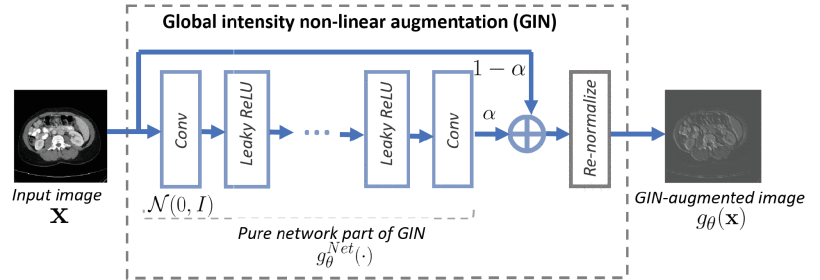
\includegraphics[width=0.9\textwidth]{figures/gin_schema.png}
    \caption{Architecture of the GIN module. © 2022 IEEE, from \cite{Ouyang2023}.}
    \label{fig:gin_schema}
\end{figure}

Then, the interventional pseudo-correlation augmentation (IPA) addresses the shifted-correlation effect, whereby background unlabeled structures $X_\mathrm{b}$ become spuriously correlated with objects of interest $X_\mathrm{f}$ due to the acquisition process. IPA approximates the causal intervention $\mathrm{do}(X_\mathrm{f}=x_\mathrm{f})$---i.e., it removes the effects of the acquisition factor $A$ on $X_\mathrm{f}$---by resampling background appearances independently of the foreground through spatially-varying assignments of appearance transforms.

Let $g_{\theta_1}$ and $g_{\theta_2}$ be two independent GIN transforms sampled for the same input image, with number of channels $C$, height $H$ and width $W$. IPA creates a low-frequency pseudo-correlation map $b\in[0,1]$ with shape $(C \times H \times W)$ and blends the two GIN outputs as
\begin{equation}\label{eq:ipa}
    T_1\bigl(x;\theta_1,\theta_2,b\bigr) = g_{\theta_1}(x) \odot b + g_{\theta_2}(x) \odot (1-b),
\end{equation}
where $\odot$ denotes the Hadamard product, that is, element-wise multiplication. A complementary view $T_2(\cdot)$ is obtained by swapping $b$ and $1-b$. Pseudo-correlation maps are generated by interpolating a lattice of randomly-valued control points with cubic B-splines; in practice the control-point spacing is set to a fraction of the image dimension $\bigl(\textrm{e.g., }\frac{1}{4}\bigr)$ to maintain low spatial frequency and avoid shape distortion (Fig.\,\ref{fig:ipa_schema}).

By applying IPA to the entire image---both background and foreground---the pipeline avoids label-induced shortcuts and approximates sampling from independent background appearance distributions. This operation can be interpreted as assigning different photometric transformations to different spatial regions so that background and foreground appearances are de-correlated across training iterations.

\begin{figure}[htbp]
    \centering
    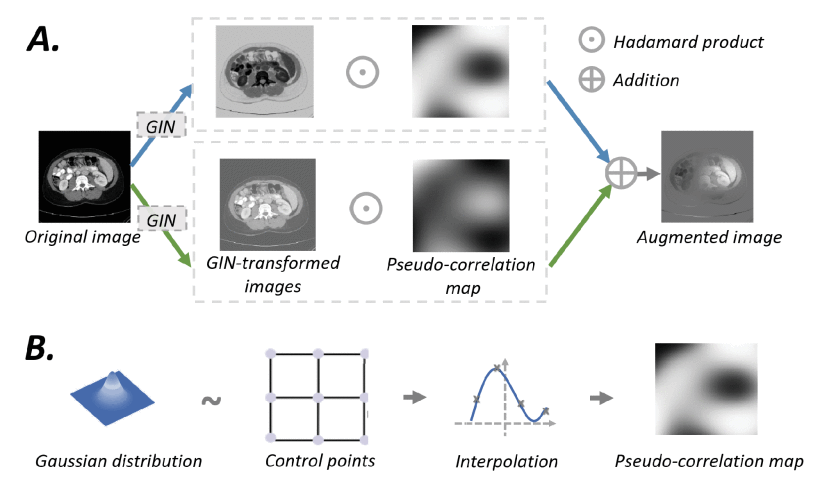
\includegraphics[width=0.9\textwidth]{figures/ipa_schema.png}
    \caption{Architecture of the IPA augmentation scheme (A), and construction principles of pseudo-correlation maps (B). © 2022 IEEE, from \cite{Ouyang2023}.}
    \label{fig:ipa_schema}
\end{figure}

In \cite{Ouyang2023} the training loop samples two GIN transforms and one pseudo-correlation map per image per iteration, generates the two IPA-augmented views $T_1(x)$ and $T_2(x)$, and computes the training loss. Alternative designs to B-spline in pseudo-correlation maps---e.g., random superpixels---were explored but found to be less effective. Both GIN and IPA steps are ruled by hyperparameters that must be set empirically. Among them, the most relevant (followed by the value that was used in \cite{Ouyang2023}, as a reference) are:
\begin{itemize}
    \item GIN
    \begin{itemize}
        \item Number of layers of the shallow network: \num{4}.
        \item Number of intermediate channels of the shallow network: \num{2}.
        \item Interpolation coefficient $\alpha$: sampled from a uniform distribution.
    \end{itemize}
    \item IPA
    \begin{itemize}
        \item Control point spacing in kernel matrix: $\frac{1}{4}\textrm{ of the image length}$; it must be small enough in order to construct low-frequency pseudo-correlation maps.
        \item Interpolation order in kernel matrix: \num{2}, it serves as smoothing factor between the control points in the pseudo-correlation map.
        \item Control point values: sampled from a Gaussian distribution.
        \item Downscale of the image: \num{2}, reduce the computational load.
    \end{itemize}
\end{itemize}
Default values were set by the authors of the paper by the combination of hyperparameter tuning, heuristic choices and hardware limitations.

Actually, practical optimizations include controlling the depth and width of the GIN networks. In \cite{Ouyang2023}, Ouyang and colleagues conducted hyperparameter tuning on the number of layers and channels in the GIN architecture, and on the sampling distribution of the interpolation coefficient $\alpha$. An ablation study on the contribution of the IPA step to the global performance was also conducted, showing improvements in all tested scenarios with respect to GIN-only training.

The proposed approach consistently yields superior performance gains compared with other methods---MixStyle\,\cite{Zhou2021}, AdvBias\,\cite{Chen2020}, RandConv\,\cite{Xu2021} and others---when tested on unseen domains across three cross-domain segmentation scenarios:
\begin{itemize}
    \item Cross-modality abdominal image segmentation (CT-MRI).
    \item Cross-sequence cardiac MRI segmentation (\textsc{bSSFP}-LGE).
    \item Cross-site prostate MRI segmentation.
\end{itemize}

Finally, Ouyang and colleagues also participated in the FeTA 2022 challenge\,\cite{FeTA2022_review}. Their approach was based on training different nnU-Net models with varying data augmentation methods. \textsc{gin-ipa} was employed in the augmentation pipeline for one of these models\,\cite{FeTA2022_top}. The models were subsequently ensembled, and the resulting segmentation method achieved the highest performance in the challenge, ranking first. GIN augmentation and \textsc{gin-ipa} were also used in three models in the FeTA 2024 challenge\,\cite{FeTA2024_review}.

\section{Evaluation Metrics}
